\chapter{模板使用示例}
\label{cha:example}

本章展示本模板的常用 \LaTeX{} 功能示例，供撰写论文时参考。

%% ====================================================================
\section{标题层级}
\label{sec:heading}
%% ====================================================================

本模板支持三级标题，格式已由模板统一设置，无需手动调整字号和间距。章标题为一级标题（三号黑体居中），节标题为二级标题（小三号黑体居左），条标题为三级标题（四号黑体居左）。

\subsection{三级标题示例}
\label{subsec:heading3}

三级标题为四号黑体，居左。一般论文写到三级标题即可，不建议使用更深的层级。

%% ====================================================================
\section{正文与引用}
\label{sec:text}
%% ====================================================================

正文为小四号宋体，行距20磅，段首缩进两个汉字。西文字体为 Times New Roman。

引用参考文献时使用 \texttt{\textbackslash cite} 命令，如：深度学习在图像识别领域取得了显著进展\cite{ref1}，目标检测算法也得到了广泛研究\cite{ref2,ref3}。

论文中对某一问题、概念、观点等的简单解释、说明、评价、提示等，如不宜在正文中出现，可采用文中编号加“脚注”的形式。
当论文中的字、词或短语，需要进一步加以说明，而又没有具体的文献来源时，用注释。注释一般在社会科学中用得较多。
应控制论文中的注释数量，不宜过多（规范§3.10.6）。注释以脚注形式呈现，使用 \texttt{\textbackslash footnote} 命令，内容自动置于当页页脚，并以编号与正文对应。例如：迁移学习\footnote{迁移学习（Transfer Learning）：将在源任务上学得的知识迁移到目标任务中，以提升目标任务的学习效果。}是近年来深度学习领域的重要研究方向。

交叉引用使用 \texttt{\textbackslash ref} 命令，如：第~\ref{sec:figure}~节展示了图的用法，表~\ref{tab:simple}~为简单表格示例，公式~(\ref{eq:euler})~为欧拉公式。

科技名词术语及设备、元件的名称，应采用国家标准或部颁标准中规定的术语或名称。标准中未规定的术语要采用行业通用术语或名称。全文名词术语必须统一。一些特殊名词或新名词应在适当位置加以说明或注解。
采用英语缩写词时，除本行业广泛应用的通用缩写词外，文中第一次出现的缩写词应该用括号注明英文原词（规范§3.10.8）。例如：卷积神经网络（Convolutional Neural Network，CNN）在图像分类任务中表现优异，后文直接使用 CNN 即可。循环神经网络（Recurrent Neural Network，RNN）适合处理序列数据，长短期记忆网络（Long Short-Term Memory，LSTM）是其常用变体。

%% ====================================================================
\section{字体样式}
\label{sec:font}
%% ====================================================================

\subsection{加粗}

正文宋体和黑体均配置了伪加粗（\texttt{AutoFakeBold}），直接使用 \texttt{\textbackslash textbf\{\}} 即可，无需切换字体：

\textbf{这是加粗的宋体文字，bold songti}

{\heiti\textbf{这是加粗的黑体文字，bold heiti}}

\subsection{斜体}

斜体主要用于西文和数学符号，中文一般不使用斜体。西文斜体使用 \texttt{\textbackslash textit\{\}}：

\textit{This is italic text. Variables like $f(x) = ax^2 + bx + c$ use italic automatically.}

\subsection{下划线}

下划线使用 \texttt{\textbackslash underline\{\}}，但长文本换行时需改用 \texttt{ulem} 宏包的 \texttt{\textbackslash uline\{\}}（本模板已加载）：

\underline{短文本下划线} \quad \uline{较长的下划线文本，uline 命令支持自动换行，适合段落中使用}

\subsection{其他常用样式}

删除线：\sout{这段文字有删除线}

上角标：正文\textsuperscript{上角标}，下角标：正文\textsubscript{下角标}


%% ====================================================================
\section{图}
\label{sec:figure}
%% ====================================================================

图应有“自明性”，尽量使用矢量图，插入pdf最佳。插图应与文字紧密配合，文图相符，内容正确。选图要力求精练，插图、照片应完整清晰。图应有图题，图题即图的名称，置于图的编号之后。
图中各部分说明应采用中文（引用的外文图除外）或数字符号，各项文字说明置于图题之上（有分图时，置于分图题之上）

\subsection{单图}

如图~\ref{fig:example}~所示为单图示例。

\begin{figure}[htbp]
    \centering
    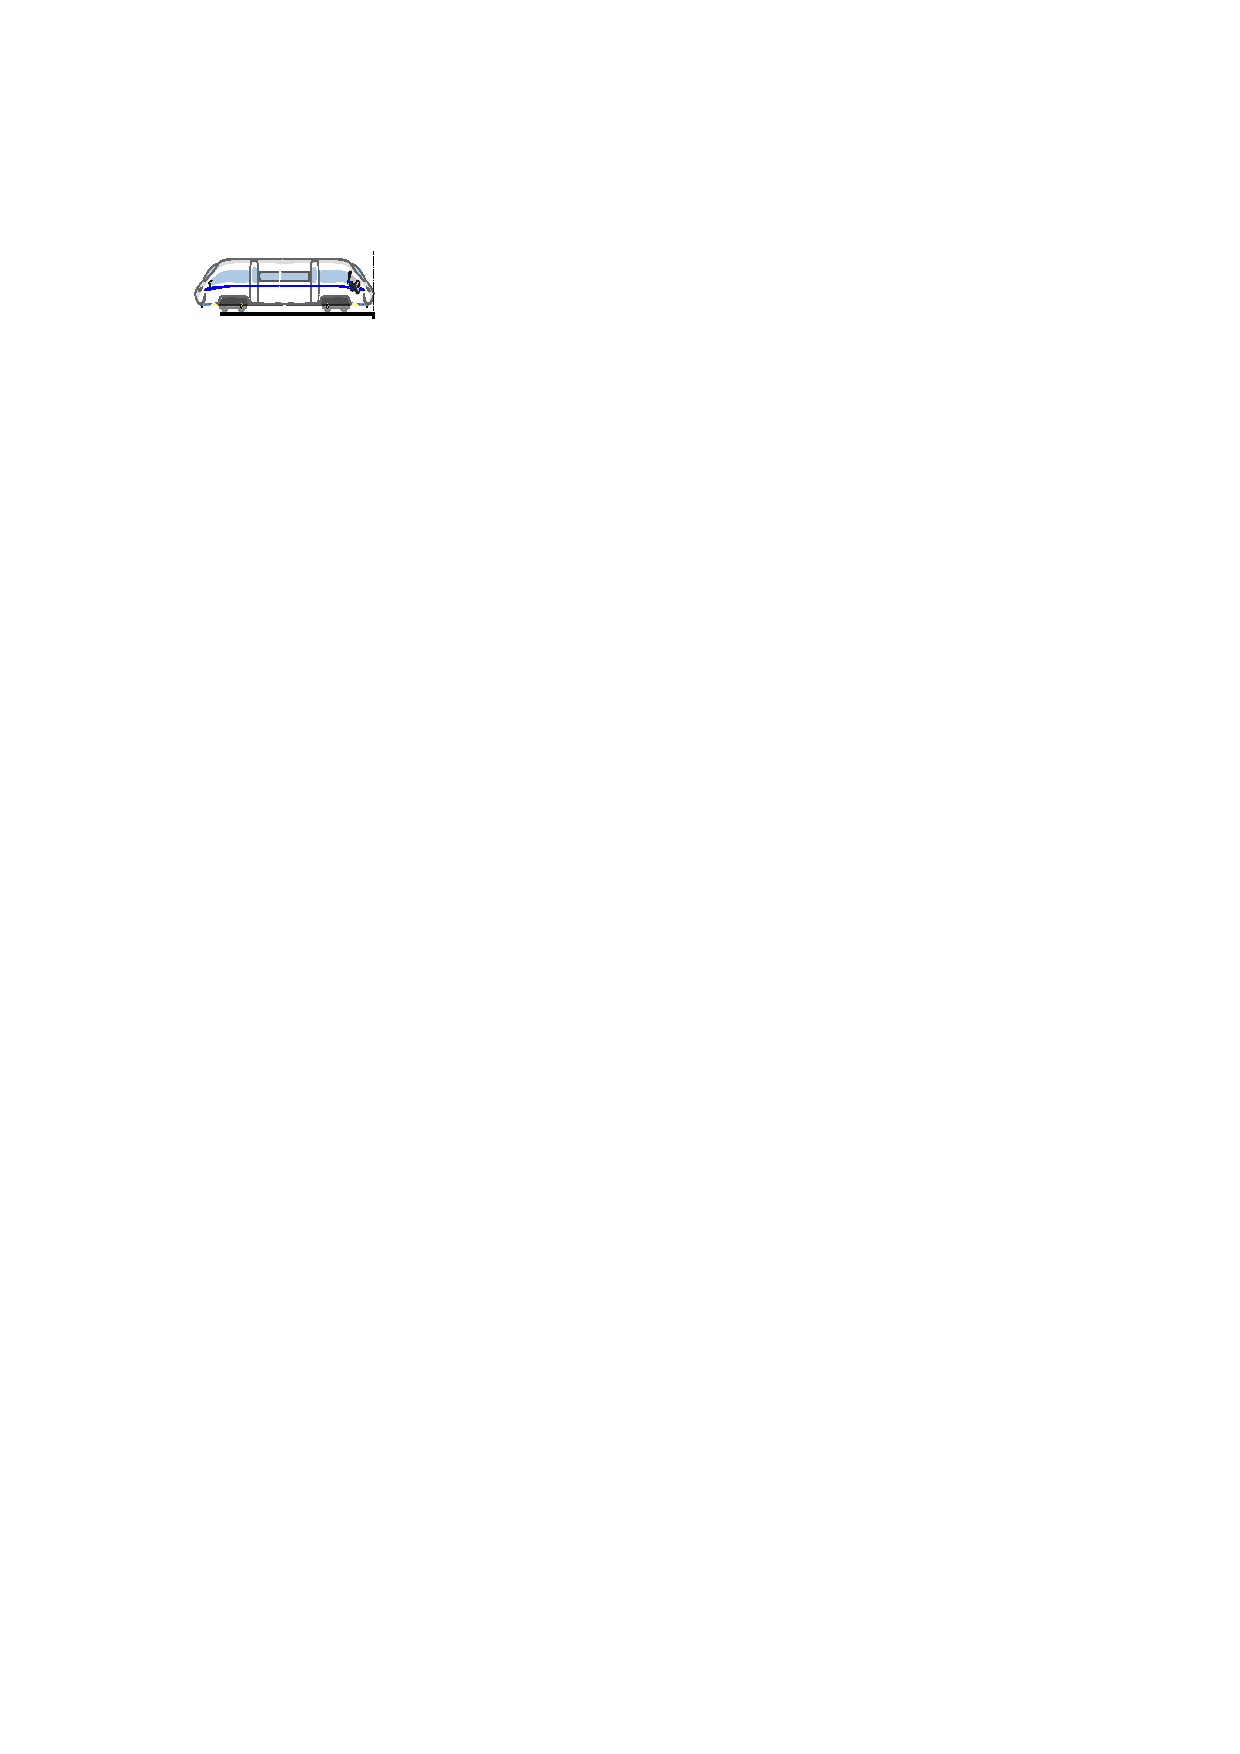
\includegraphics[width=0.5\textwidth]{figures/figure1}
    \figcaption{单图示例}{Single Figure Example}
    \label{fig:example}
\end{figure}

\subsection{并排子图}

分图号用 a)、b) 等表示，分图题置于分图之下，用中英文书写，如图~\ref{fig:subfig}~所示。

\begin{figure}[htbp]
    \centering
    \begin{subfigure}[b]{0.45\textwidth}
        \centering
        \includegraphics[width=\textwidth]{example-image-a}
        \subfigcaption{子图示例一}{Subfigure Example One}
        \label{fig:subfig_a}
    \end{subfigure}
    \hfill
    \begin{subfigure}[b]{0.45\textwidth}
        \centering
        \includegraphics[width=\textwidth]{example-image-b}
        \subfigcaption{子图示例二}{Subfigure Example Two}
        \label{fig:subfig_b}
    \end{subfigure}
    \figcaption{并排子图示例}{Subfigure Example}
    \label{fig:subfig}
\end{figure}

%% ====================================================================
\section{表}
\label{sec:table}
%% ====================================================================

插表之前文中必须有相关文字提示，表题置于表的上方，采用中英文对照，表与上下文字间需空一行编排（规范§3.10.5）。

\subsection{基本三线表}

如表~\ref{tab:simple}~所示为基本三线表。

\begin{table}[htbp]
    \centering
    \tabcaption{基本三线表示例}{Example of Basic Three-Line Table}
    \label{tab:simple}
    \begin{tabular}{cccc}
        \toprule
        \textbf{方法} & \textbf{精度（\%）} & \textbf{召回率（\%）} & \textbf{F1（\%）} \\
        \midrule
        方法A & 92.3 & 89.1 & 90.7 \\
        方法B & 93.5 & 91.2 & 92.3 \\
        方法C & \textbf{95.1} & \textbf{93.4} & \textbf{94.2} \\
        \bottomrule
    \end{tabular}
\end{table}

\subsection{全表同一单位}

全表使用同一单位时，将单位符号移至表头右上角并加圆括号（规范§3.10.5），如表~\ref{tab:unit}~所示。

\begin{table}[htbp]
    \centering
    \tabcaption{各方法运行时间对比}{Comparison of Running Time for Each Method}
    \label{tab:unit}
    \begin{tabular}{ccc}
        \toprule
        \textbf{方法} & \textbf{训练时间（h）} & \textbf{推理时间（ms）} \\
        \midrule
        方法A & 12.3 & 45.2 \\
        方法B & 8.6  & 32.1 \\
        方法C & 6.1  & 21.8 \\
        \bottomrule
    \end{tabular}
\end{table}

\subsection{含空缺数据的表格}

表中数字空缺的格内加横线“--”（占2个半角字符）。表内文字或数字上、下或左、右相同时，不允许用“〃”、“同上”之类的写法（规范§3.10.5），如表~\ref{tab:missing}~所示。

\begin{table}[htbp]
    \centering
    \tabcaption{含空缺数据的表格示例}{Table Example with Missing Data}
    \label{tab:missing}
    \begin{tabular}{cccc}
        \toprule
        \textbf{数据集} & \textbf{方法A} & \textbf{方法B} & \textbf{方法C} \\
        \midrule
        数据集一 & 92.3 & 89.1 & 90.7 \\
        数据集二 & 92.3 & --   & 92.3 \\
        数据集三 & --   & 91.2 & --   \\
        \bottomrule
    \end{tabular}
\end{table}

\subsection{引用他人表格}

引用文献中的表格时，须在中英文表题右上角标注参考文献序号（规范§3.10.5），如表~\ref{tab:cited}~所示。

\begin{table}[htbp]
    \centering
    \tabcaption{引用他人表格示例\textsuperscript{\cite{ref1}}}{Table Example Cited from Reference\textsuperscript{\cite{ref1}}}
    \label{tab:cited}
    \begin{tabular}{ccc}
        \toprule
        \textbf{类别} & \textbf{数量} & \textbf{比例（\%）} \\
        \midrule
        类别A & 120 & 40.0 \\
        类别B & 180 & 60.0 \\
        \bottomrule
    \end{tabular}
\end{table}

\subsection{含文字说明的表格}

表内文字说明起行空2个半角字符，转行顶格，句末不加标点（规范§3.10.5），如表~\ref{tab:note}~所示。

\begin{table}[htbp]
    \centering
    \tabcaption{含文字说明的表格示例}{Table Example with Text Notes}
    \label{tab:note}
    \begin{tabular}{cp{0.45\textwidth}c}
        \toprule
        \textbf{编号} & \multicolumn{1}{c}{\textbf{说明}} & \textbf{数值} \\
        \midrule
        1 & {\hangindent=1em\hangafter=1\hspace{1em}该方法采用卷积神经网络提取特征，结合注意力机制提升精度} & 92.3 \\
        2 & {\hangindent=1em\hangafter=1\hspace{1em}基于Transformer结构，训练数据量较大，推理速度较慢，但精度显著优于其他方法} & 95.1 \\
        \bottomrule
    \end{tabular}
\end{table}

\subsection{跨页续表}

一般情况下插表不能拆开两页编排，确实排不下时才转页，以续表形式接排。续表右上角注明编号后加“（续表）”，并重复表头（规范§3.10.5），如表~\ref{tab:longtable}~所示。

\setlength{\LTleft}{0pt plus 1fill}
\setlength{\LTright}{0pt plus 1fill}
\begin{longtable}{ccccc}
    \tabcaption{跨页续表示例}{Example of Multi-Page Table} \label{tab:longtable} \\
    \toprule
    \textbf{序号} & \textbf{名称} & \textbf{数值A} & \textbf{数值B} & \textbf{数值C} \\
    \midrule
    \endfirsthead
    %% 续页：右上角”表X-X（续表）”，重复表头
    \multicolumn{5}{r}{表~\thetable（续表）} \\
    \toprule
    \textbf{序号} & \textbf{名称} & \textbf{数值A} & \textbf{数值B} & \textbf{数值C} \\
    \midrule
    \endhead
    \bottomrule
    \endfoot
    \bottomrule
    \endlastfoot
    1  & 项目一  & 0.123 & 1.234 & 2.345 \\
    2  & 项目二  & 0.234 & 1.345 & 2.456 \\
    3  & 项目三  & 0.345 & 1.456 & 2.567 \\
    4  & 项目四  & 0.456 & 1.567 & 2.678 \\
    5  & 项目五  & 0.567 & 1.678 & 2.789 \\
    6  & 项目六  & 0.678 & 1.789 & 2.890 \\
    7  & 项目七  & 0.789 & 1.890 & 2.901 \\
    8  & 项目八  & 0.890 & 1.901 & 2.012 \\
    9  & 项目九  & 0.901 & 2.012 & 3.123 \\
    10 & 项目十  & 1.012 & 2.123 & 3.234 \\
    11 & 项目十一 & 1.123 & 2.234 & 3.345 \\
    12 & 项目十二 & 1.234 & 2.345 & 3.456 \\
    13 & 项目十三 & 1.345 & 2.456 & 3.567 \\
    14 & 项目十四 & 1.456 & 2.567 & 3.678 \\
    15 & 项目十五 & 1.567 & 2.678 & 3.789 \\
\end{longtable}

%% ====================================================================
\section{数学公式}
\label{sec:equation}
%% ====================================================================

\subsection{行内公式}

行内公式使用 \texttt{\$...\$}，如：设 $f(x) = ax^2 + bx + c$，其中 $a \neq 0$。公式中物理量、符号用斜体。

\subsection{独立编号公式}

%% 规范§3.10.12：公式另行居中，编号置于括号内右端对齐，格式为”（章-序号）”
%% 文中引用公式用”见式（X-X）”或”由公式（X-X）”
独立编号公式使用 \texttt{equation} 环境，公式编号格式为”（章-序号）”。欧拉公式如式~(\ref{eq:euler})~所示：

\begin{equation}
    e^{i\pi} + 1 = 0
    \label{eq:euler}
\end{equation}

\subsection{公式前说明文字}

%% 规范§3.10.12：公式前有说明文字（如”解”、”假定”等），文字前空4个半角字符，公式仍居中
若公式前有说明文字（如“解”、“假定”等），文字前空4个半角字符（\texttt{\textbackslash quad}），公式仍居中书写，公式末不加标点。

\hspace{2em}解\quad

\begin{equation}
    x = \frac{-b \pm \sqrt{b^2 - 4ac}}{2a}
    \label{eq:quadratic}
\end{equation}

\subsection{长公式转行}

%% 规范§3.10.12：较长公式应在”=”处或”+””-””×””/”处回行
较长的公式应尽可能在等号处回行，使用 \texttt{align} 环境对齐等号；也可在”$+$””$-$””$\times$””$/$”等记号处回行：

\begin{align}
    f(x) &= ax^4 + bx^3 + cx^2 + dx + e                                        \label{eq:poly} \\
         &= x^2(ax^2 + bx + c)                                                  \notag \\
         &\quad + dx + e                                                         \notag
\end{align}

\subsection{多公式组}

%% 规范§3.10.12：两个以上公式从”1”开始编号，公式较多时可分章编排
麦克斯韦方程组由式~(\ref{eq:maxwell1})至式~(\ref{eq:maxwell4})给出：

\begin{align}
    \nabla \cdot \mathbf{E}  &= \frac{\rho}{\varepsilon_0}                             \label{eq:maxwell1} \\
    \nabla \cdot \mathbf{B}  &= 0                                                       \label{eq:maxwell2} \\
    \nabla \times \mathbf{E} &= -\frac{\partial \mathbf{B}}{\partial t}                \label{eq:maxwell3} \\
    \nabla \times \mathbf{B} &= \mu_0\mathbf{J} + \mu_0\varepsilon_0
                                \frac{\partial \mathbf{E}}{\partial t}                 \label{eq:maxwell4}
\end{align}

\subsection{分数线与行内分数}

%% 规范§3.10.12：分数线长度应等于或略大于分子分母中较长的一方；
%% 正文行内分数应降低高度：将上下分数写成”/”形式，或将根号改为负指数

正文行内书写分数时，应将高度降为一行。例如，将 $\dfrac{1}{\sqrt{2}}$ 写成 $1/\sqrt{2}$ 或 $2^{-1/2}$。

\subsection{除法表示}

%% 规范§3.10.12：用斜线表示”除”时应加括号避免含糊，”乘”的关系在前
公式中用斜线表示”除”的关系时应采用括号，以免含糊不清，如 $a/(b\cos x)$。通常”乘”的关系在前，如 $a\cos x/b$ 而不写成 $(a/b)\cos x$。


%% ====================================================================
\section{列表}
\label{sec:list}
%% ====================================================================

正文中的标号按规范§3.10.2规定的顺序排列：先 (1)(2)(3)，再 1)~2)~3)，后 \Circled{1}~\Circled{2}~\Circled{3}，标号后避免出现标点符号或项目符号。多层级嵌套示例如下：

\begin{enumerate}[label=(\arabic*)]
    \item 数据准备
    \begin{enumerate}[label=\arabic*)]
        \item 原始数据采集
        \begin{enumerate}[label=\Circled{\arabic*}]
            \item 传感器数据读取
            \item 网络爬虫抓取
        \end{enumerate}
        \item 数据清洗与去噪
        \item 数据集划分，训练集与测试集比例为 8:2
    \end{enumerate}
    \item 模型设计与训练
    \begin{enumerate}[label=\arabic*)]
        \item 选取网络结构，设置学习率为 $1\times10^{-3}$
        \item 设计损失函数，训练轮数为 100
    \end{enumerate}
    \item 结果评估与分析，采用精度、召回率等指标进行衡量
\end{enumerate}

%% ====================================================================
\section{代码}
\label{sec:code}
%% ====================================================================

代码使用 \texttt{lstlisting} 环境，示例如下。（无官方模板）

\begin{lstlisting}[language=Python]
import numpy as np

def softmax(x):
    """计算 softmax"""
    e_x = np.exp(x - np.max(x))
    return e_x / e_x.sum()

if __name__ == '__main__':
    logits = np.array([1.0, 2.0, 3.0])
    print(softmax(logits))
\end{lstlisting}

%% ====================================================================
\section{算法}
\label{sec:algorithm}
%% ====================================================================

算法使用 \texttt{algorithm} 和 \texttt{algorithmic} 环境，示例见算法~\ref{alg:example}。

\begin{algorithm}[htbp]
    \caption{梯度下降算法}
    \label{alg:example}
    \begin{algorithmic}[1]
        \Require 学习率 $\alpha$，最大迭代次数 $T$，初始参数 $\theta_0$
        \Ensure 优化后的参数 $\theta$
        \State $\theta \leftarrow \theta_0$
        \For{$t = 1, 2, \ldots, T$}
            \State 计算梯度 $g_t \leftarrow \nabla_\theta \mathcal{L}(\theta)$
            \State 更新参数 $\theta \leftarrow \theta - \alpha \cdot g_t$
            \If{$\|g_t\| < \varepsilon$}
                \State \textbf{break}
            \EndIf
        \EndFor
        \State \Return $\theta$
    \end{algorithmic}
\end{algorithm}

%% ====================================================================
\section{参考文献引用}
\label{sec:citation}
%% ====================================================================
尽量引用原始文献。当不能引用原始文献时，要将二次引用文献、原始文献同时标注。

博士学位论文的参考文献一般不少于100篇，学术型硕士学位论文的参考文献一般不少于50篇，专业硕士学位论文的参考文献一般不少于30篇，其中外文文献一般不少于总数的1/2。参考文献中近五年的文献数一般应不少于总数的1/3，并应有近两年的参考文献和一定数量的学位论文或专业名著。

产品说明书、未公开发表的研究报告（著名的内部报告如PB、AD报告及著名大公司的企业技术报告等除外）以及其它无法通过公开途径获得的文献资料通常不宜作为参考文献引用。

引用网上参考文献时，应注明该文献的准确网页地址，网上参考文献和各类标准不包含在上述规定的文献数量之内。本人在攻读学位期间发表的学术论文不应列入参考文献中。


引用标注遵照 GB/T 7714-2005，采用顺序编码制（规范§3.10.7）。引用文献的标示置于所引内容最后一个字的右上角，编号用阿拉伯数字置于方括号中，以上角标形式标注。

\subsection{基本引用}

引用单篇文献时，编号置于引用内容末尾右上角，如：深度学习在图像识别领域取得了显著进展\cite{ref1}。

\subsection{同一处引用多篇文献}

同一处引用多篇文献时，各序号在方括号内全部列出，遇连续序号可标注讫序号，如：相关研究表明该方法具有较好的泛化能力\cite{ref1,ref2,ref3}，也可写成连续形式\cite{ref1,ref4,ref5,ref6}。

\subsection{多次引用同一文献}

多次引用同一文献时，在序号的方括号后标注引文页码（规范§3.10.7），使用 \texttt{\textbackslash cite[页码]\{key\}} 实现，如：电场对激子的解离作用已有详细论述\cite[15-19]{ref1}，其主要结论\cite[25-27]{ref1}在后续研究中得到了广泛验证。

\subsection{文献序号作为正文成分}

当参考文献为文中直接说明时，序号与正文排齐（非上角标），使用 \texttt{\textbackslash parencite} 命令，如：由文献\parencite{ref3}可知，该算法的时间复杂度为 $O(n\log n)$；连续序号形式如：文献\parencite{ref1,ref3,ref4,ref5}对此有详细论述。

\subsection{各类文献引用示例}

本节依次引用规范§3.11所列各类文献类型：

\begin{itemize}
    \item 期刊论文\cite{ref1,ref2,ref3}：作者.文章题目[J].期刊名,年份,卷号(期数):页码.
    \item 著作\cite{ref4,ref5}：作者.书名[M].出版地:出版社,年份.
    \item 会议论文\cite{ref6}：作者.文章名[C].//编者.论文集名,会议地址,会议时间.出版地:出版者,年份.
    \item 学位论文\cite{ref7}：作者.题名[D].保存地点:保存单位,年份.
    \item 专利\cite{ref8}：申请者.专利题名[P].国别,专利号.发布日期.
    \item 技术标准\cite{ref9}：起草责任者.标准代号.标准名称.出版地:出版者,年份.
    \item 报纸\cite{ref10}：作者.题名[N].报纸名,出版日期(版次).
    \item 电子文献\cite{ref11}：作者.题名[EB/OL].发布年.[引用日期].网址.
\end{itemize}

注意：不得将引用文献标示置于各级标题处。


